\documentclass[3p,times,procedia]{elsarticle}
\flushbottom

\usepackage{ecrc}
\usepackage[bookmarks=false]{hyperref}
\hypersetup{hidelinks}

\usepackage{amsmath}
\usepackage{amssymb,amsfonts}
\usepackage{graphicx}
\usepackage{textcomp}
\usepackage{xcolor}
\usepackage{booktabs}
\usepackage{multirow}
\usepackage{url}
\usepackage{acronym}
\usepackage[section]{placeins}

\volume{00}
\firstpage{1}
\journalname{Procedia Computer Science}
\runauth{A. Gargouri et al.}
\jid{procs}

\acrodef{hrc}[HRC]{Human-Robot Collaboration}
\acrodef{tcn}[TCN]{Temporal Convolutional Network}
\acrodef{tta}[TTA]{Test-Time Augmentation}
\acrodef{imu}[IMU]{Inertial Measurement Unit}
\acrodef{gpu}[GPU]{Graphics Processing Unit}
\acrodef{cv}[CV]{Cross-Validation}
\acrodef{mlp}[MLP]{Multilayer Perceptron}
\acrodef{ffn}[FFN]{Feed-Forward Network}
\acrodef{bn}[BN]{Batch Normalization}
\acrodef{ln}[LN]{Layer Normalization}
\acrodef{gelu}[GELU]{Gaussian Error Linear Unit}
\acrodef{dwconv}[DWConv]{Depthwise Convolution}
\acrodef{fp}[FP]{False Positives}
\acrodef{fn}[FN]{False Negatives}

\begin{document}
\begin{frontmatter}

    \dochead{30th International Conference on Knowledge-Based and Intelligent Information \& Engineering Systems (KES 2026)}

    \title{Danger-State Detection in Human-Robot Collaboration Using Deep Learning}

    \author[a,b]{Ameur Gargouri}
    \author[b]{Mohamed Karray*}
    \author[a]{Mohamed Ksantini}

    \address[a]{ATISP Lab, ENET'Com, University of Sfax, Sfax, Tunisia}
    \address[b]{ESME Research Lab, Ivry-sur-Seine, France}
    %add a one/two sentences about my own work
    \begin{abstract}
        Collaborative robots operating in shared workspaces present inherent physical hazards, such as unexpected high-impact collisions, clamping and crushing forces. Deploying these robots in human proximity requires continuous monitoring via sensors to prevent operator injury and production interruptions. A core challenge in this context is the false-alarm trade-off: sensor outputs often lead to frequent emergency stops that erode productivity and operator trust. Current methods solve this problem either through the use of expensive force/torque sensors, visual processing pipelines, or shallow learning; nevertheless, no systematic analysis of current deep learning methods has been performed yet. To address these limitations, we propose, in this paper, a deep learning pipeline for binary danger-state classification (safe vs.\ danger) from high-frequency wearable \ac{imu} data recorded during physical \ac{hrc}.  The proposed approach is based on three main components: (1) GPU-based feature expansion
        that computes velocity and acceleration from raw position data, creating 195 input channels without requiring extra
        force sensors; (2) a systematic comparison of five 1D deep learning architectures; and (3) a post-processing stage
        designed specifically to reduce false alarms. Evaluated with five-fold stratified cross-validation from 60 subjects, ConvNeXt 1D and Temporal Convolutional Network (TCN) demonstrate the best macro-F1 results (98.68\% and 98.62\% correspondingly), with the danger precision over 98\% and danger recall over 97\%. The post-processing stage alone reduces false positives by 87.5\% at a cost of only 1.2 percentage points in recall, establishing a safer operating point for industrial deployment.
    \end{abstract}

    \begin{keyword}
        human-robot collaboration \sep danger detection \sep temporal convolutional network \sep deep learning \sep wearable sensors \sep post-processing
    \end{keyword}

\end{frontmatter}

\newpage
ConvNeXt~1D and \ac{tcn} achieve the highest macro-F1 scores (98.68\% and 98.62\%, respectively), with danger precision exceeding 98\% and recall above 97\%.

%===================================================================
\section{Introduction}
\label{sec:introduction}
%===================================================================

\Ac{hrc} refers to shared-workspace scenarios in which a human operator and a robotic arm coordinate physical actions toward a common objective~\cite{selvaggio2021autonomy}. In these situations, it becomes imperative for the robot to keep on assessing whether the state of ongoing interaction is safe or whether there is a threat looming that calls for precautionary measures. Failing to detect a threatening situation could result in an injury, while false warnings could halt the process. This balance between sensitivity and specificity forms a key issue within safety in industry under ISO/TS 15066~\cite{iso15066}.

Current collision detection methods can be broadly categorized into three families. Hardware-dependent approaches rely on dedicated force-torque sensors or six-dimensional force transducers to measure contact forces directly~\cite{wang2025sixdof}. Observer-based methods employ mathematical state estimators, such as Extended State Observers, to infer external forces from joint-level measurements without additional sensors~\cite{tonti2024eso}. Data-driven approaches train classifiers on sensor recordings, using signal transformations such as wavelet decompositions~\cite{niu2024wavelet} or multivariate fusion~\cite{fang2024multivariate} to improve discriminability. More recently, digital twin environments have been proposed to simulate collision scenarios for safer algorithm development~\cite{an2024digitaltwin} and deep learning has been integrated with zero-force control strategies~\cite{zhao2025zeroforce}.

Despite these developments, some challenges remain. First, the force/torque sensing mechanism is an added expense and mechanical complication. The observer scheme requires a precise dynamic model, which is difficult to guarantee in reality. Most data-driven techniques used presently rely on shallow neural networks or wavelet analysis of features. Furthermore, the false-alarm problem, whereby noisy sensor outputs lead to unnecessary emergency stops, remains insufficiently addressed in the literature.

This paper addresses these gaps by proposing a deep learning pipeline that operates on wearable \ac{imu} data collected during physical \ac{hrc}. Rather than relying on six-dimensional force sensors~\cite{wang2025sixdof} or external cameras~\cite{hoang2024grasp}, the pipeline introduces a \ac{gpu}-accelerated kinematic feature expansion that computes velocity and acceleration on the fly, augmenting the 65-channel \ac{imu} input to 195 spatio-temporal features and thereby encoding physical dynamics without additional hardware cost. Where recent collision detection studies have relied on wavelet networks~\cite{niu2024wavelet}, basic deep learning~\cite{zhao2025zeroforce}, or mathematical observers~\cite{tonti2024eso}, this work systematically benchmarks five next-generation architectures originally designed for computer vision: \ac{tcn}, ConvNeXt~1D, MLP-Mixer~1D, Transformer~1D and InceptionTime, adapted to one-dimensional time-series safety classification under identical training and evaluation conditions. To further improve prediction reliability, \ac{tta} is applied at inference time, a technique that remains virtually unexplored in the robotic collision literature despite its proven benefits in other domains~\cite{fang2024multivariate}. Finally, a temporal debouncing post-processor applies a three tap median filter coupled with the optimal thresholding value in order to target the false-alarm productivity trade-off, reducing false positives by 87.5\% while preserving danger precision above 95\%. All experiments are conducted through a rigorous five-fold stratified cross-validation on over 69,000 real-world windows from 60 subjects, providing a level of statistical robustness that digital twin simulations~\cite{an2024digitaltwin} alone cannot guarantee.
%first, second,...

The remainder of this paper is organized as follows. Section~2 reviews related work on collision detection and safety monitoring in \ac{hrc}. Section~3 describes the proposed methodology, including data preprocessing, model architectures, training protocol and post-processing. Section~4 presents the experimental results and discussion. Section~5 concludes with implications and future directions.

%===================================================================
\section{Related Work}
\label{sec:related}
%===================================================================

Safety monitoring in \ac{hrc} has been addressed through sensor-based detection, model-based estimation and data-driven classification~\cite{khan2026safety}. This section reviews recent contributions in each direction, highlighting the specific limitations that motivate the present work.

Direct force-torque measurement remains a foundational approach for physical collision monitoring. In this domain, Wang et al.~\cite{wang2025sixdof} proposed a collision detection and force compensation framework based on a six-dimensional force sensor mounted at the robot end-effector. Their method achieves accurate contact localization by directly measuring interaction forces along all six degrees of freedom. However, the reliance on a dedicated force-torque transducer adds significant hardware cost and calibration complexity, limiting scalability in multi-robot production lines where each arm would require its own sensor suite.

Extending physical interaction monitoring to specialized robot topologies, Gao et al.~\cite{gao2024cable} investigated collision detection in cable-driven parallel robots, a domain where conventional joint-level sensing is unavailable. Their approach uses cable tension variations to determine the interactions between the human user and the cable assembly. While successful in its own right due to the specific geometry of the cable assembly robot, the algorithm is only suited to serial-link cobots and needs tension sensors which are not typically found in industrial cobots.

To eliminate external hardware, model-based disturbance estimation has gained traction. Specifically, Tonti et al.~\cite{tonti2024eso} introduced a fast collision detection system based on an Extended State Observer (ESO) that reconstructs disturbance forces from joint-level position and velocity measurements without external sensors. Through the ESO method, an estimate of the disturbance signal is generated, which includes all of the unmodelled system dynamics, making it possible to detect collision through the application of the residual threshold method. The main strength of this method is that no additional hardware needs to be installed, but the performance depends on how well the nominal dynamic model of the robot is defined.

Integrating compliant robot control with learning-based detection represents another research direction. Work by Zhao et al.~\cite{zhao2025zeroforce} combined zero-force control with deep learning to detect collisions while maintaining compliant robot behavior. Their framework trains a neural network to distinguish between intentional contact forces arising from the collaborative task and unexpected collision forces. The integration of compliance control with collision detection is a notable contribution, but the method relies on joint torque signals that are not always available on low-cost cobots and the deep learning component is limited to a basic architecture without comparison to modern alternatives.

From a data-driven perspective, multi-modal signal aggregation has been explored to boost detection robustness. Fang et al.~\cite{fang2024multivariate} presented a multivariate collision detection algorithm based on fusion of signals from different types of sensors like motor current values, joint angles, and accelerometers used during dynamic \ac{hrc} operations. The fusion strategy leverages complementary information across modalities, achieving robustness to individual sensor noise. However, the classification backend relies on conventional signal processing and shallow models and the study does not evaluate modern deep architectures that could learn richer cross-modal representations directly from the raw fused signals.

Focusing on time-frequency signal decomposition, Niu et al.~\cite{niu2024wavelet} introduced Continuous Wavelet Networks (CWNet) that extract features from joint-level signals for efficient and transferable collision detection across different collaborative robots. The wavelet decomposition provides a principled multi-resolution representation of transient collision events and the authors demonstrate transfer learning between robot platforms. Nevertheless, the wavelet-based feature extraction constitutes a fixed preprocessing step that may discard discriminative patterns not captured by the chosen wavelet basis and the network architecture does not explore recent convolutional designs such as \ac{tcn} or ConvNeXt.

Rather than reacting after physical contact occurs, vision-based proactive planning aims to prevent collisions entirely. Hoang et al.~\cite{hoang2024grasp} addressed safety from a planning perspective by utilizing color and depth images to generate collision-free grasp trajectories before execution. Their vision-based pipeline evaluates candidate grasps against a reconstructed scene model, rejecting those that would result in contact with obstacles or the human operator. While proactive trajectory planning is complementary to reactive collision detection, this approach requires a calibrated RGB-D camera with a clear line of sight and cannot handle unforeseen events that occur during task execution.

Virtual workspace simulation has also emerged as a means to benchmark safety protocols safely offline. In this context, An et al.~\cite{an2024digitaltwin} developed a digital twin framework for offline collision analysis within \ac{hrc} workspaces, enabling algorithm evaluation in a simulated environment before physical deployment. The digital twin copies both the kinematics of the robot and the workspace geometry in order to create synthetic collision situations that can be used to train and validate collision detection algorithms. Despite reducing the dangers involved with testing in the physical domain, simulation environments have been shown to lack the stochastic nature of human behavior, sensor noise, and other variables inherent in actual collisions.

In summary, prior work highlights the need for data-driven safety monitors that can achieve high precision without expensive hardware or complex dynamic models. A systematic comparison of modern deep architectures on high-frequency kinematic data, combined with temporal post-processing to mitigate false alarms, has not been reported. The present work directly addresses this gap.

%===================================================================
\section{Methodology}
\label{sec:methodology}
%===================================================================

The proposed solution follows the pipeline summarized in Figure~\ref{fig:overview}. Raw IMU data is preprocessed, expanded via GPU-accelerated derivatives, passed through 1D deep learning classifiers and finally stabilized using a temporal debouncing post-processor.

\begin{figure}[!h]
    \centering
    
\includegraphics[width=1.0\columnwidth]{fig1_pipeline_overview.pdf}
    \caption{Proposed deep learning pipeline for danger-state detection in human-robot collaboration.}
    \label{fig:overview}
\end{figure}

\subsection{Problem Formulation}

Danger-state detection is formulated as a binary classification problem on sliding-window segments of multimodal \ac{imu} recordings. Let $\mathbf{X}_i \in \mathbb{R}^{C \times T}$ denote a window of $T$ time steps across $C$ sensor channels, with binary label $y_i \in \{0, 1\}$ indicating safe ($y_i{=}0$) or danger ($y_i{=}1$). A window is labeled as danger if any constituent time step carries a danger annotation, enforcing a conservative labeling policy:
\begin{equation}
    y_i = \max_{t \in \{1,\ldots,T\}} y_i^{(t)}
\end{equation}
Given a model $f_\theta$, the predicted class probability is $p_\theta(y{=}1 \mid \mathbf{X}_i)$. The predicted label is obtained by thresholding this probability at a tuned operating point $\tau$:
\begin{equation}
    \hat{y}_i = \mathbf{1}\left[p_\theta(y{=}1 \mid \mathbf{X}_i) > \tau\right]
\end{equation}

\subsection{Data Collection and Dataset}

All experiments in this work are evaluated on the DASIG (Dataset of Standard and Abrupt Industrial Gestures) benchmark~\cite{dasig2024}, a standard corpus collected in a simulated industrial workstation to study human motion dynamics relevant to safety in human-robot collaboration scenarios. The dataset comprises high-frequency inertial recordings from 60 healthy adult subjects (36 males and 24 females, aged 20 to 59) performing simulated industrial pick-and-place tasks. Each subject completed three structured trials, generating complete interaction sequences that capture natural variability across body morphologies, movement speeds and motor strategies.

Motion data were acquired at a sampling rate of 200~Hz using five wireless APDM Opal Magneto-Inertial Measurement Units (MIMUs)~\cite{apdm_opal}. The five sensors were placed on key upper-body anatomical landmarks to capture upper-limb kinematics and torso motion: Sternum (STR), Right Upper Arm (RUA), Right Forearm (RFA), Left Upper Arm (LUA) and Left Forearm (LFA), as illustrated in Figure~\ref{fig:sensorplacement}.

Each MIMU outputs 13 kinematic variables per time step: tri-axial linear acceleration ($\mathbf{a} \in \mathbb{R}^3$), tri-axial angular velocity ($\boldsymbol{\omega} \in \mathbb{R}^3$), tri-axial magnetic field intensity ($\mathbf{m} \in \mathbb{R}^3$) and a four-component orientation quaternion ($\mathbf{q} \in \mathbb{R}^4$). Across all five sensors, each window yields $5 \times 13 = 65$ synchronized input channels.
\begin{figure}[!h]
    \centering
    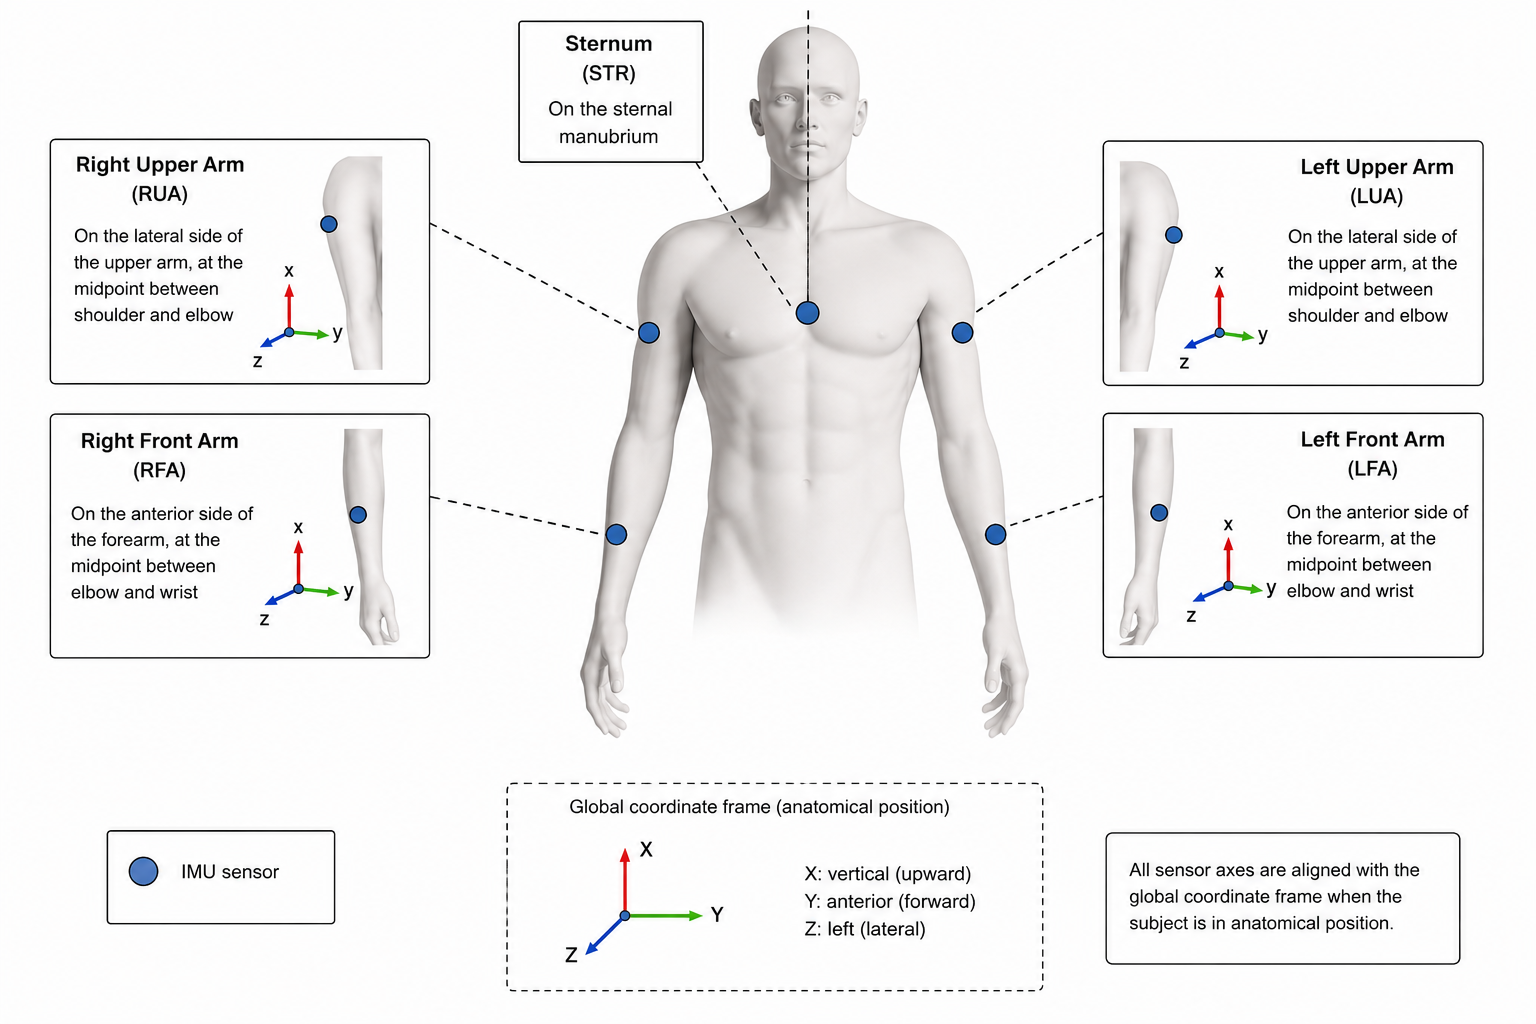
\includegraphics[width=1.0\columnwidth]{ChatGPT Image Jul 29, 2026, 04_01_33 PM.png}
    \caption{Anatomical placement of the five wireless MIMU sensors during the DASIG data collection experiments.}
    \label{fig:sensorplacement}
\end{figure}

During each trial, subjects executed 30 standard pick-and-place gestures interleaved with four abrupt evasive movements (two triggered by visual alarms and two by acoustic alarms). Each trial is accompanied by a separate Arduino event log that records the temporal instants and numeric codes of all stimuli: codes 2-5 correspond to green LED activations at stations SA-SD (standard gestures), codes 6-9 to red LED activations (visual alarms) and code 10 to acoustic buzzer activations.

The DASIG data set consists of 180 recording files individually (60 subjects $\times$ 3 trials). Each file forms a time series matrix with about 18,000 rows (time steps at 200~Hz over $\sim$90~s) and 66 columns, where one timestamp column is followed by 65 columns of sensor data ($5~\text{MIMUs} \times 13~\text{variables}$). Event log files contain multi-class labeling information for events (green light, red light, or buzzer) along with the exact timestamps and station identifiers. For the purpose of this work, we derive a binary classification target by mapping all alarm-triggered events (codes 6-10) to the \textit{danger} class and the remaining standard gestures to the \textit{safe} class.

\subsection{Data Preprocessing and Dynamic Feature Expansion}

Preprocessing transforms the raw DASIG recordings into a fixed-size tensor representation suitable for deep learning classifiers, proceeding through three sequential stages, as illustrated in Figure~\ref{fig:datapipeline}. First, raw recordings are segmented into windows of 0.5~s duration (100 time steps) with 50\% overlap, producing 69,094 labeled windows. Second, each window is normalized per trial using z-score standardization:
\begin{equation}
    x_{\text{norm}} = \frac{x - \mu_{\text{trial}}}{\sigma_{\text{trial}}}
\end{equation}
where $\mu_{\text{trial}}$ and $\sigma_{\text{trial}}$ are computed from the training partition of the corresponding trial. Third, window-level labels are assigned using the conservative maximum policy defined in Section~\ref{sec:methodology}: a window is labeled as danger if any constituent time step carries a danger annotation. The resulting dataset exhibits a class imbalance of 87.6\% safe (60,559 windows) and 12.4\% danger (8,535 windows).



Instead of relying entirely on positional data, the pipeline shown in Figure~\ref{fig:datapipeline} performs preprocessing of each window by adding the first and second derivatives of the positional information in time via finite differences:
\begin{equation}
    \mathbf{V}_i = \frac{d\mathbf{X}_i}{dt}, \quad \mathbf{A}_i = \frac{d^2\mathbf{X}_i}{dt^2}
\end{equation}
The expanded representation $[\mathbf{X}_i; \mathbf{V}_i; \mathbf{A}_i] \in \mathbb{R}^{3C \times T}$ yields $3 \times 65 = 195$ channels which represent position, velocity, and acceleration. The augmentation process takes place on the \ac{gpu} during training and testing. This removes the need for any kind of offline storage, as well as provides the network with kinematics information about human movements.
\begin{figure}[!h]
    \centering
    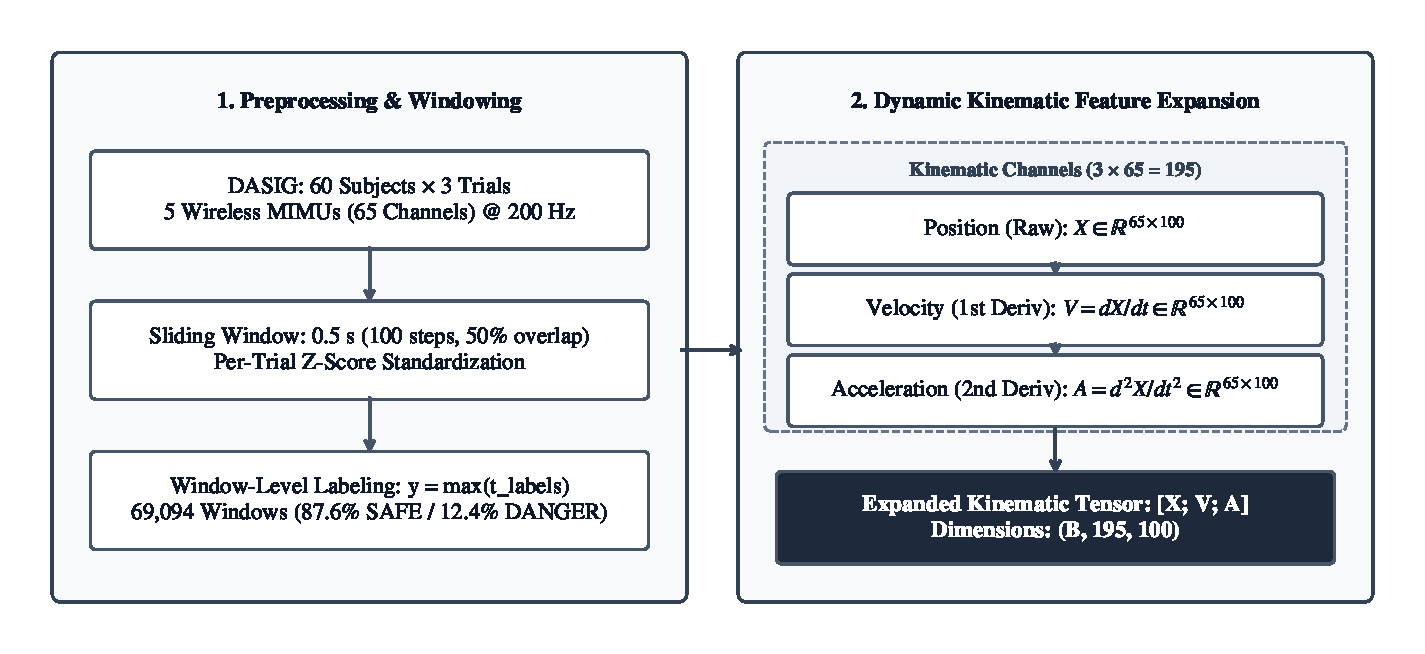
\includegraphics[width=1.0\columnwidth]{fig2_data_pipeline.pdf}
    \caption{Data preprocessing and dynamic feature expansion on the GPU.}
    \label{fig:datapipeline}
\end{figure}
\FloatBarrier

\subsection{Algorithm Selection}

Early iterations of this pipeline employed classical machine learning models, including Random Forest and XGBoost, trained on hand-crafted statistical features (mean, variance, skewness, kurtosis) extracted from each window. While these models achieved reasonable accuracy on the original 65-channel representation, they exhibited two fundamental limitations when applied to the expanded 195-channel kinematic input.

First, classical models operate on fixed-length feature vectors and therefore require an explicit feature engineering stage that collapses the temporal dimension. This aggregation discards the sequential ordering of time steps within each window, which is precisely where safety-critical transitions manifest: a sudden acceleration spike spanning only a few consecutive frames can distinguish a dangerous impact from normal motion. Second, the combinatorial growth of potential cross-channel interactions across 195 features makes manual feature design intractable and tree-based models cannot exploit the spatial locality of sensor groups (e.g., adjacent joint channels) without domain-specific feature grouping.

These observations motivated the transition to deep learning architectures that operate directly on the raw $(C \times T)$ tensor without manual feature extraction. Deep models learn hierarchical representations that jointly capture temporal dynamics and cross-channel correlations, eliminating the information loss inherent in statistical summarization.

In the domain of deep learning, our design choice includes architecture selection to incorporate three different types of inductive biases for a well-rounded comparison: (1) convolutional networks (TCN and ConvNeXt 1D) using local temporal dependencies through sliding windows and dilated receptive fields; (2) MLP-type networks (MLP-Mixer 1D) capturing global token and channel relationships in an unsupervised way without relying on convolution or attention; and (3) attention networks (Transformer 1D) utilizing self-attention to model long-range relationships. InceptionTime is considered as a multi-scale convolutional architecture often used for time series classification tasks. This combination includes the main architectural classes possible for sequential problems and allows us to draw conclusions on the inductive bias most suited for high-frequency kinematic safety signals.
%\subsection{Model Architectures}

Five architectures are adapted from their original two-dimensional formulations to operate on one-dimensional time-series input of shape $(B, 195, 100)$, where $B$ is the batch size:

\textbf{\ac{tcn}}~\cite{bai2020tcn}: A stack of six dilated causal convolutional blocks with kernel size 3 and exponentially increasing dilation factors ($d = 1, 2, 4, 8, 16, 32$), preceded by a $1{\times}1$ projection from 195 to 256 channels. Residual connections and batch normalization are applied in each block.

\textbf{ConvNeXt~1D}~\cite{liu2022convnext}: Four ConvNeXt layers which use depthwise separable convolution with kernel size 7 and inverted bottlenecks inspired by the two-dimensional network structure. Strided stem layer with kernel size 3 converts input channels from 195 to 128.

\textbf{MLP-Mixer~1D}~\cite{tolstikhin2021mlpmixer}: Four mixer layers that use token-mixing and channel-mixing MLPs. The input is projected into 128-dimensional tokens via a patch embedding layer with kernel size 5 and stride 5.

\textbf{Transformer~1D}~\cite{vaswani2017attention}: A four-layer encoder having four attention heads and a feed forward layer dimensionality of 256 along with learned positional encodings. The linear projection of the 195 input channels gives 128 dimensions.

\textbf{InceptionTime}~\cite{fawaz2020inceptiontime}: Two inception modules with parallel convolutions at kernel sizes 1, 3 and 5 plus max-pooling, followed by adaptive average pooling.

All architectures terminate with adaptive average pooling, layer normalization and a linear classifier producing two-class logits.

\subsection{Training Protocol}

All models share an identical training protocol to ensure that performance differences reflect architectural properties rather than optimization variations. The training objective is focal loss~\cite{lin2017focal} with focusing parameter $\gamma = 2.0$ and label smoothing $\epsilon = 0.01$:
\begin{equation}
    \mathcal{L}_{\text{focal}} = -\frac{1}{N} \sum_{i=1}^{N} w_{y_i} (1 - p_\theta(y_i \mid \mathbf{X}_i))^\gamma \log p_\theta(y_i \mid \mathbf{X}_i)
\end{equation}
where $w_c$ denotes the inverse-frequency class weight for class $c$. Optimization uses AdamW~\cite{loshchilov2019adamw} with learning rate $10^{-3}$, weight decay $10^{-4}$ and OneCycleLR scheduling~\cite{smith2019onecycle}. Gradient norms are clipped to 1.0. Batch size is 128 and training runs for 30 epochs. A weighted random sampler balances mini-batch class composition.

Data augmentation combines three strategies: (1) scale jitter that randomly scales each channel by a factor drawn from $\mathcal{U}(0.95, 1.05)$; (2) additive Gaussian noise with $\sigma = 0.01$; and (3) Mixup~\cite{zhang2018mixup} with probability 0.3 and mixing coefficient $\alpha = 0.1$ drawn from a Beta distribution.

\subsection{Evaluation Strategy}

Model evaluation employs five-fold stratified cross-validation, which helps maintain the same class balance in each fold. On average, each fold contains around 55,275 training samples and 13,819 validation samples. The checkpoint with the highest macro-F1 during the validation process is selected as the optimal model.

\ac{tta} is applied at inference time: a validation sample is run through the model four times (once normally and three times with Gaussian noise) to obtain the final score by averaging the softmax probabilities obtained from each pass.

Reported metrics include accuracy, macro-F1, danger recall (sensitivity) and danger precision. Confusion matrices are row-normalized to facilitate comparison across models.

\subsection{Temporal Post-Processing}

Raw model predictions are refined through two sequential post-processing steps designed to suppress transient false alarms without sacrificing detection latency.

First, a median filter of kernel size 3 is applied to the sequence of predicted danger probabilities. This temporal smoothing eliminates isolated high-confidence predictions that arise from sensor noise or brief ambiguous motions.

Second, the decision threshold $\tau$ is optimized by sweeping over $[0.50, 0.95]$ in increments of 0.01 and selecting the value that maximizes danger precision subject to the constraint that danger recall remains above 95\%. The resulting threshold $\tau = 0.77$ yields a substantial reduction in false positives. The impact of this temporal post-processing is illustrated in Figure~\ref{fig:postprocess}.

\begin{figure}[!h]
    \centering
    
\includegraphics[width=1.0\columnwidth]{fig5_evaluation_postprocessing.pdf}
    \caption{Temporal debouncing and threshold optimization on model probabilities.}
    \label{fig:postprocess}
\end{figure}

%===================================================================
\section{Results and Discussion}
\label{sec:results}
%===================================================================

\subsection{Comparison}

Table~\ref{tab:results} presents the benchmark results for all five architectures after temporal post-processing (median filter and $\tau = 0.77$). Models are ranked by macro-F1 score.

\begin{table}[h!]
    \caption{Benchmark results with temporal post-processing ($\tau = 0.77$, median-filtered)}
    \label{tab:results}
    \centering
    \footnotesize
    \setlength{\tabcolsep}{3pt}
    \begin{tabular}{@{}clcccc@{}}
        \toprule
        \textbf{Rank} & \textbf{Model} & \textbf{Accuracy} & \textbf{Macro-F1} & \textbf{Danger Recall} & \textbf{Danger Precision} \\
        \midrule
        1             & ConvNeXt 1D    & 99.43\%           & 98.68\%           & 97.13\%                & 98.25\%                   \\
        2             & TCN            & 99.41\%           & 98.62\%           & 97.14\%                & 98.04\%                   \\
        3             & MLP-Mixer 1D   & 99.28\%           & 98.32\%           & 95.88\%                & 98.27\%                   \\
        4             & InceptionTime  & 98.30\%           & 96.22\%           & 97.53\%                & 89.62\%                   \\
        5             & Transformer 1D & 96.47\%           & 92.50\%           & 95.85\%                & 79.71\%                   \\
        \bottomrule
    \end{tabular}
\end{table}

This demonstrates a clear order of performance in terms of CNN architectures (ConvNeXt 1D and TCN) performing best, followed by the mixed architecture (MLP-Mixer 1D), while the attention-only Transformer 1D obtains the poorest performance. Such an order is consistent with the well-known inductive bias of convolution operations in learning local temporal features from sequential data, which are common in kinematic danger signals.

ConvNeXt~1D achieves the highest macro-F1 (98.68\%) with 148 false positives and 245 false negatives across 69,094 windows (see Figure~\ref{fig:cm}). The TCN obtains nearly identical macro-F1 (98.62\%), but with a slightly greater number of false positives (166). Both models provide macro-F1 above 98\%, which means that less than 2\% of the dangers are false positives.

\begin{figure}[!h]
    \centering
    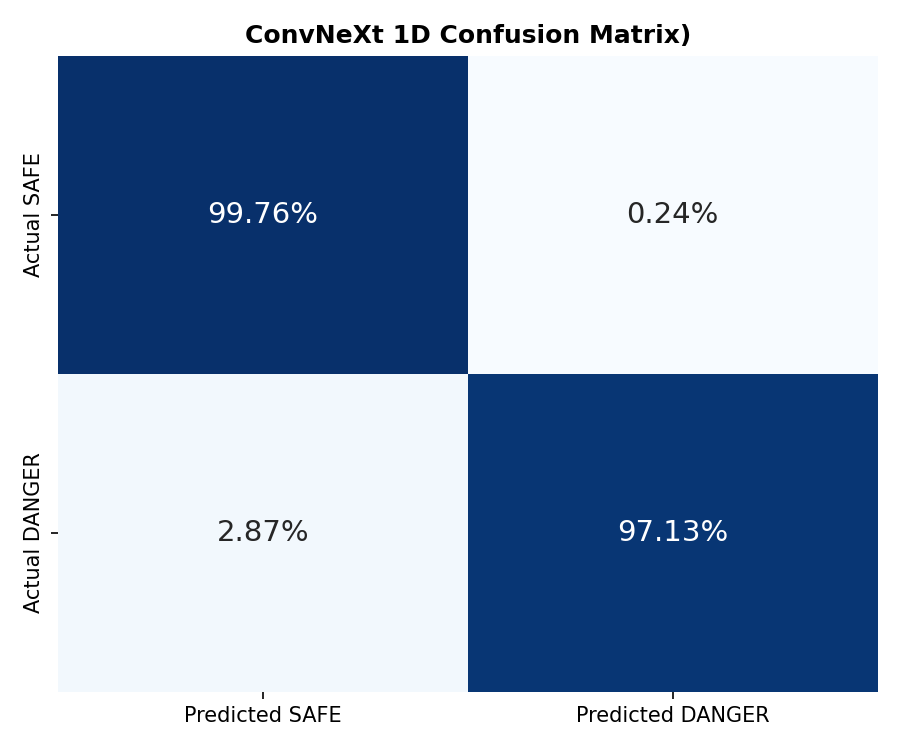
\includegraphics[width=0.6\columnwidth]{ConvNeXt_1D_cm.png}
    \caption{Row-normalized confusion matrix for the best-performing ConvNeXt 1D model.}
    \label{fig:cm}
\end{figure}

The MLP-Mixer 1D model demonstrates a precision of 98.27\%, whereas its recall is 95.88\%, thus revealing an omission rate of roughly 4\% for actual dangerous cases. It corresponds to the patch-wise tokenization used in the mixer model, which might fail to recognize detailed temporal changes at the boundaries between patches.

InceptionTime provides an excellent recall of 97.53\%, yet it has significantly lower precision of 89.62\%, which leads to 964 false positives. The multi-resolution parallel convolution mechanism used in the inception cell can successfully detect broader temporal trends, yet it produces more boundary uncertainties.

The Transformer~1D model, despite strong recall (95.85\%), suffers from the lowest precision (79.71\%) and produces 2,082 false positives. The quadratic attention mechanism, while powerful for capturing long-range dependencies, appears to lack the local inductive bias necessary for the short, structured temporal patterns that characterize safety-critical transitions in \ac{imu} data.

\subsection{Impact of Temporal Post-Processing}

Table~\ref{tab:postprocess} quantifies the effect of the median filter and threshold tuning on the \ac{tcn} model, comparing raw model output (threshold 0.50) against the post-processed configuration.

\begin{table}[h!]
    \caption{Effect of temporal post-processing on TCN predictions}
    \label{tab:postprocess}
    \centering
    \footnotesize
    \setlength{\tabcolsep}{4pt}
    \begin{tabular}{@{}lcccc@{}}
        \toprule
        \textbf{Configuration}          & \textbf{FP} & \textbf{FN} & \textbf{Precision} & \textbf{Recall} \\
        \midrule
        Raw output ($\tau = 0.50$)      & 1,324       & 142         & 83.9\%             & 98.3\%          \\
        + Median filter + $\tau = 0.77$ & 166         & 244         & 98.0\%             & 97.1\%          \\
        \midrule
        \textbf{Relative change}        & $-$87.5\%   & +71.8\%     & +14.1 pp           & $-$1.2 pp       \\
        \bottomrule
    \end{tabular}
\end{table}

Temporal post-processing reduces false positives by 87.5\% (from 1,324 to 166) at the cost of a modest 1.2 percentage point decrease in recall (from 98.3\% to 97.1\%). This trade-off is favorable for industrial deployment, where each false positive triggers an unnecessary emergency stop that disrupts production flow.

\subsection{Discussion}

The experimental results support three observations relevant to danger-state detection in \ac{hrc}.

First, CNN-based architectures with dilated or depthwise convolutions provide a strong inductive bias for kinematic time-series classification. The local receptive fields of convolutional filters align naturally with the temporal structure of motion data, where safety-critical transitions occur over short, contiguous intervals. This finding contrasts with the recent trend toward attention-based models in other domains and suggests that architecture selection should be guided by the temporal characteristics of the target signal.

Second, dynamic feature expansion from 65 to 195 channels provides the network with explicit velocity and acceleration information that would otherwise need to be learned implicitly. This design choice eliminates the need for expensive force-torque sensors while achieving precision levels (above 98\%) that approach the reliability of hardware-based approaches reported in the literature~\cite{wang2025sixdof}.

Third, temporal post-processing addresses the false-alarm problem that is widely acknowledged but rarely solved quantitatively in the \ac{hrc} safety literature. The median filter suppresses isolated false detections caused by sensor noise, while the optimized threshold shifts the operating point toward higher precision without sacrificing operational safety. This two-stage approach is model-agnostic and can be applied to any probabilistic safety classifier.

%===================================================================
\section{Conclusion}
\label{sec:conclusion}
%===================================================================

Using collaborative robots in shared workspaces requires a careful balance between safety and productivity. Safety systems must detect genuine hazards to protect human operators, but frequent false alarms cause unnecessary emergency stops that slow down production and reduce operator trust.

To solve the problem stated above, this paper suggests a deep learning pipeline for online danger state detection utilizing the data from wearable sensors. The pipeline consists of three main parts: (1) feature expansion based on GPU-acceleration that allows obtaining the velocity and acceleration features from the position data and providing 195 input channels without requiring any force sensors; (2) comparison of five different one-dimensional deep learning models; and (3) post-processing aimed at reducing the number of false alarms.

The experimental evaluation with five-fold cross-validation on the DASIG dataset shows that convolutional models, namely, ConvNeXt 1D and TCN networks, give the best results with macro-F1 scores more than 98.6\%. It is noteworthy that post-processing reduces the rate of false alarms by 87.5\%, leading to danger precision higher than 98.0\% and maintaining danger detection recall above 97.1\%. Thus, it has been proven that the combination of wearable sensors and deep learning can ensure safe monitoring of human-robot cooperation without using expensive equipment.

In the future, the research plans further testing of the pipeline on unseen subjects, lightweight architectures analysis, and embedded implementation of the models to meet the requirements of real-time safety monitoring according to the ISO/TS 15066.
\newpage
\bibliographystyle{elsarticle-num}
\bibliography{cobot_safety_references}

\end{document}
